\documentclass[a5paper]{article}
\usepackage{graphicx}
\usepackage{hyperref}
\usepackage[parfill]{parskip}% don't indent new sections
\usepackage[utf8]{inputenc}
\usepackage[a4paper]{geometry}
\pagestyle{empty}


\title{Sum of Degrees Squared}
\author{Emil Lynegaard}

\begin{document}
  \maketitle
  \section{Experiment}
  For this experiment, the programming language Go will be used. The experiment will set out to compare sorting of a list of numbers with a priority queue and with a call to a library sort function. Since Go does not ship with a priority queue directly, an implementation thereof from their documentation of their heap package\footnote{\url{https://golang.org/pkg/container/heap/}} will be used. The sort function that will be used is Go's \texttt{sort.Ints}\footnote{\url{https://golang.org/pkg/sort/\#Ints}}.

\textbf{Measurement:} For the comparison, the experiment will be ran 100 times for both the priority queue and for the library sort function. The input will be of size \texttt{5.000.000} and the two experiments will be ran independently on the same machine with minimal process interference.

\textbf{Assumption:} Due to the nature of a priority queue, it has additional housekeeping to do when we inserting and deleting items from it. Therefore we will claim that the library sorting function, will sort and return our input faster than the priority queue.

\section{Results}
\begin{figure}[!ht]
    \centering
    \noindent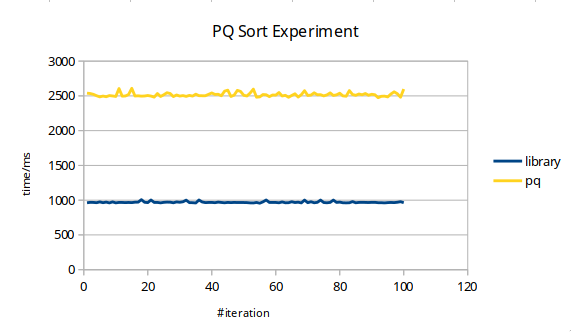
\includegraphics[scale=0.6]{graph.png}
    \caption{Graph plotting the running times of PQ-sort and Library-sort.}
    \label{fig:graph}
\end{figure}

Based on our results shown in Figure~\ref{fig:graph}, we can with a certainty of 95\% say that for permuting a list \texttt{A} to give a result \texttt{B} such that \texttt{B} is sorted\footnote{Sorted in this case meaning B[i] $\le$ B[i+1] for any i.}, the priority queue implementation has at most a 0.69071\% chance of being faster or equally fast as the library function.\footnote{What a bold statement. Is this even remotely close to the intended experiment?}. This is given the following:
\[ {(1-p_{H})}^{100} \le.05 \]
\[ p_{H}\ge 1-.05^{1/100} \]
\[ p_{H}\ge 691/10.000 \]

From Figure~\ref{fig:graph} we may also observe that the standard deviation for both the library function and for the priority queue is relatively small, while the distance between the two methodologies remain very large, indicating that the actual chance of the priority queue outperforming the library is even smaller estimated. 

\section{Bonus question}
The priority queue will never be faster at sorting an array than a sensible library function. This is due to the overhead of maintaining the advantageous data structure that most priority queues will have. However, if one was fine with keeping the data in the priority queue, and had to repeatedly insert new items into the data structure, a priority queue would vastly outperform a basic array. For the priority queue we would get insertions of $O(\log n)$ in contrast to $O(n)$ with a naive array implementation..
\end{document}
